% !TEX root = main.tex

\section{优化算法}
\subsection{简介}
\begin{example}
\begin{mini*}
    {}{f_0(\vx)}{}{}
    \addConstraint{A\vx}{=\vb}
\end{mini*}
\end{example}
\begin{analysis}
1$\degree$ 罚函数法(penalty function)
\[\min F(\vx):=f_0(\vx)+\frac{\lambda}{2}\norm{A\vx-\vb}_2^2\]
\[\tilde{\vx}=\argmin_\vx F\implies\nabla f_0(\tilde{\vx})+\lambda A^\T(A\tilde{\vx}-\vb)=0\]
2$\degree$ 拉格朗日函数方法
\[\begin{aligned}
    \qquad&L(\vx,\vv)=f_0(\vx)+\vv^\T(A\vx-\vb)\\
    \implies& g(\vv)=\inf_\vx \lrp{f_0(\vx)+\vv^\T(A\vx-\vb)}\\
    \qquad& \vv=\lambda(A\tilde{\vx}-\vb)\\
    \implies & g(\lambda(A\tilde{\vx}-\vb))=\inf_\vx \lrp{f_0(\vx)+\lambda(A\tilde{\vx}-\vb)^\T(A\vx-\vb)}
\end{aligned}\]
\end{analysis}

\begin{example}
\begin{mini*}
    {}{f_0(\vx)}{}{}
    \addConstraint{A\vx}{\geq\vb}
\end{mini*}
\end{example}
\begin{analysis}
log-barrier函数
\[\min f_0(\vx)+\sum_{i=1}^m u_i\log(a_i^\T \vx-b_i)\]
\end{analysis}


考虑这样的问题,$f_0(\vx)$可微,凸,无约束,即
\begin{mini*}
    {}{f_0(\vx)}{}{}
\end{mini*}
\begin{enumerate}
    \item 所有算法都是迭代的
    \[\iter{\vx}{k+1}=\iter{\vx}{k}+\iter{\alpha}{k}\iter{\vd}{k}\]
    $\alpha\geq 0$为步长,$\vd$为方向,所有算法本质上都是选择方向与步长的问题
    \item 如何选择步长$\iter{\alpha}{k}$
    \[\begin{cases}
    \text{确定步长} & \begin{cases}\text{固定步长}\\\text{变化步长(递减步长)}\end{cases}\\
    \text{搜索步长}
    \end{cases}\]
    最优步长:线搜索问题,给定当前点及方向
    \[\iter{\alpha}{k}=\argmin_{\alpha\geq 0} f_0(\iter{\vx}{k}+\alpha\iter{\vd}{k})\]
    \begin{enumerate}
        \item 黄金分割法(0.618法)/优选法求解线搜索问题:这样做的采样复杂度很低,之前算过的点很容易被再用!
        \item 不精确线搜索(Armijo Rule)/回溯直线搜索:一阶泰勒展开
        \begin{algorithm}[H]
            \caption{不精确线搜索}
            \begin{algorithmic}[1]
                \State{$\iter{\alpha}{k}=\alpha_{\text{max}},\mu\in(0,1/2)$}
                \If{$f_0(\iter{\vx}{k}+\iter{\alpha}{k}\iter{\vd}{k})>f_0(\iter{\vx}{k})+\mu\iter{\alpha}{k}\lrang{\nabla f_0(\iter{\vx}{k}),\iter{\vd}{k}}$}
                \State $\iter{\alpha}{k+1}\gets\iter{\alpha}{k}\beta,\beta\in(0,1)$
                \Else
                \State Stop
                \EndIf
            \end{algorithmic}
        \end{algorithm}
    \end{enumerate}
    而实际上没有必要求最优步长,在该方向上的差异并没有太大
    \item 关键问题是选方向
\end{enumerate}

而针对不同的优化问题,核心关键点都在于\textcolor{red}{求解KKT条件}!

\subsection{梯度下降法}
取$\iter{\vd}{k}=-\nabla f_0(\iter{\vx}{k})$,则迭代格式为
\[\iter{\vx}{k+1}=\iter{\vx}{k}-\iter{\alpha}{k}\nabla f(\iter{\vx}{k})\]

关注下面几个问题
\begin{itemize}
    \item 能否收敛
    \item 收敛到哪里
    \item 收敛速度
\end{itemize}

\subsubsection{前提假设}
\begin{itemize}
    \item[0.] 基本假设:$f$为可微的凸函数,
    \[\vx^\star=\argmin_\vx f_0(\vx)\]
    存在且有限,$f_0(\vx^\star)$有限
    \item[1.] Lipschitz连续梯度\footnote{一些基本性质可见\url{https://xingyuzhou.org/blog/notes/Lipschitz-gradient}}
    \[\exists L\geq 0,\forall \vx,\vy:\;\norm{\nabla f_0(\vx)-\nabla f_0(\vy)}\leq L\norm{\vx-\vy}\]
    等价定义:
    \begin{itemize}
        \item[a.]若$f_0(\vx)$二阶可微
    \[\forall \vx:\;\nabla^2f_0(\vx)\preceq LI\]
        \item[b.] 下界
    \[\lrang{\nabla f_0(\vx)-\nabla f_0(\vy),\vx-\vy}\geq\frac{1}{L}\norm{\nabla f_0(\vx)-\nabla f_0(\vy)}^2\]
        \item[c.] 上界
    \[\lrang{\nabla f_0(\vx)-\nabla f_0(\vy),\vx-\vy}\leq L\norm{\vx-\vy}^2\]
        \item[d.] 当函数为凸时
    \[0\leq f_0(\vy)-f_0(\vx)-\lrang{\nabla f_0(\vx),\vy-\vx}\leq\frac{L}{2}\norm{\vx-\vy}_2^2\]
    \end{itemize}
    \item[2.] 强凸性(strong convexity):即加了正则化项
    \[\exists\mu>0,\forall \vx,\vy:\;f_0(\vy)\geq f_0(\vx)+\lrang{\nabla f_0(\vx),\vy-\vx}+\frac{\mu}{2}\norm{\vx-\vy}_2^2\]
    二阶可微情况下的等价定义
    \[\nabla^2 f(\vx)\succeq \mu I\]
\end{itemize}
\begin{example}
    判断下列函数是否符合Lipschitz连续梯度及强凸性条件
    \[\begin{aligned}
        f_0(\vx) &= \vone^\T \vx\qquad & L &= 0 & \text{\xmark}\\
        f_0(\vx) &= \frac{1}{2}\norm{\vx}_2^2 & L &=1 & \mu=1\\
        f_0(\vx) &= \frac{1}{4}\norm{\vx}_2^4 & \text{\xmark} & &\text{\xmark}
    \end{aligned}\]
\end{example}

区别于严格凸(strictly convex),强凸一定是严格凸

\begin{theorem}
    严格凸函数只有一个最小值点
\end{theorem}
\begin{analysis}
    反证法,假设$\vx,\vy$均为最小值点,且$\vx\ne \vy$
    \[f_0(\vy)>f_0(\vx)+\lrang{\nabla f_0(\vx),\vx-\vy}=f_0(\vx)\]
    与$f_0(\vy)$的最小值矛盾
\end{analysis}

\begin{theorem}
    若$f_0(\vx)$有Lipschitz连续梯度,常数$L$,若$\alpha\in(0,\frac{2}{L})$,则有
    \[\begin{aligned}
        \forall \vx^\star:\;f_0(\iter{\vx}{k})-f_0(\vx^\star)&\leq \frac{2(f_0(\iter{\vx}{0})-f_0(\vx^\star))\norm{\iter{\vx}{0}-\vx^\star}^2}
        {2\norm{\iter{\vx}{0}-\vx^\star}^2+k\alpha(2-L\alpha)(f_0(\iter{\vx}{0})-f_0(\vx^\star))}
    \end{aligned}\]
    即以$O(\frac{1}{k})$速度收敛
\end{theorem}
\begin{analysis}
    $1\degree$ 点的单调性:与任意$\vx^\star$的距离在缩小
    \[\forall \vx^\star:\;\norm{\iter{\vx}{k+1}-\vx^\star}^2\leq\norm{\iter{\vx}{k}-\vx^\star}^2\]
    \[\begin{aligned}
        LHS &= \norm{\iter{\vx}{k}-\vx^\star-\alpha\nabla f_0(\iter{\vx}{k})}^2\\
        &=\norm{\iter{\vx}{k}-\vx^\star}^2-2\alpha\lrang{\iter{\vx}{k}-\vx^\star,\nabla f_0(\vx^k)}+\alpha^2\norm{\nabla f_0(\iter{\vx}{k})}\\
        &\leq \norm{\iter{\vx}{k}-\vx^\star}^2+\alpha(\alpha-\frac{2}{L})\norm{\nabla f_0(\iter{\vx}{k})}^2\qquad\text{注意到$\nabla f_0(\vx^\star)=0$,利用Lipschitz连续梯度}\\
        &\leq \norm{\iter{\vx}{k}-\vx^\star}^2
    \end{aligned}\]
    $2\degree$ 函数值的单调性:$f_0(\iter{\vx}{k+1})\leq f_0(\iter{\vx}{k})$(注意下降可能非常缓慢,并不一定收敛)
    \[\begin{aligned}
        f_0(\iter{\vx}{k+1})&\leq f_0(\iter{\vx}{k})+\lrang{\nabla f_0(\iter{\vx}{k}),\iter{\vx}{k+1}-\iter{\vx}{k}}+\frac{L}{2}\norm{\iter{\vx}{k+1}-\iter{\vx}{k}}^2\\
        &= f_0(\iter{\vx}{k})-\alpha\lrp{1-\frac{L\alpha}{2}}\norm{\nabla f_0(\iter{\vx}{k})}^2\\
        &\leq f_0(\iter{\vx}{k})
    \end{aligned}\]
    $3\degree$ 函数值的充分下降(即证明收敛性)
    \[f_0(\iter{\vx}{k+1})-f_0(\vx^\star)\leq f_0(\iter{\vx}{k})-f_0(\vx^\star)-\omega\norm{\nabla f_0(\iter{\vx}{k})}^2\]
    \[\begin{aligned}
        f_0(\iter{\vx}{k})-f_0(\vx^\star)&\leq \lrang{f_0(\iter{\vx}{k}),\iter{\vx}{k}-\vx^\star}\\
        &=\lrang{\nabla f_0(\iter{\vx}{k})-\nabla f_0(\vx^\star),\iter{\vx}{k}-\vx^\star}\\
        &\leq\norm{\nabla f_0(\iter{\vx}{k})-\nabla f_0(\vx^\star)}\norm{\iter{\vx}{k}-\vx^\star}\qquad\mbox{Cauchy}\\
        &\leq \norm{\nabla f_0(\iter{\vx}{k})}\norm{\iter{\vx}{k}-\vx^\star}
    \end{aligned}\]
    \[\begin{aligned}
        \iter{\Delta}{k+1}&\leq \iter{\Delta}{k}-\frac{\omega}{\norm{\iter{\vx}{0}-\vx^\star}^2}(\iter{\Delta}{k})^2\\
        \frac{1}{\iter{\Delta}{k+1}}&\leq\frac{1}{\iter{\Delta}{k+1}}-\frac{\omega}{\norm{\iter{\vx}{0}-\vx^\star}^2}\frac{\iter{\Delta}{k}}{\iter{\Delta}{k+1}}
    \end{aligned}\]
    错位相消可得结论$O(\frac{1}{k})$收敛速度
\end{analysis}

\begin{theorem}
    若$f_0$有Lipschitz连续梯度,常数$L$,强凸函数$n$,步长$\alpha\in(0,\frac{2}{\mu+L}]$,则
    \[\norm{\iter{\vx}{k}-\vx^\star}^2\leq\lrp{1-\frac{2\alpha\mu L}{\mu+L}}^k\norm{\iter{\vx}{0}-\vx^\star}^2\]
\end{theorem}
\begin{analysis}
\[\begin{aligned}
    \norm{\iter{\vx}{k}-\vx^\star}^2 &= \norm{\iter{\vx}{k}-\alpha\nabla f_0(\iter{\vx}{k})-\vx^\star}^2\\
    &= \norm{\iter{\vx}{k}-\vx^\star}^2-2\alpha\lrang{\iter{\vx}{k}-\vx^\star,\nabla f_0(\iter{\vx}{k})}+\alpha^2\norm{\nabla f_0(\iter{\vx}{k})}^2\\
    &\leq \norm{\iter{\vx}{k}-\vx^\star}^2-\frac{2\alpha}{\mu+L}\norm{\nabla f_0(\vx)}^2+\alpha^2\norm{\nabla f_0(\iter{\vx}{k})}^2 \qquad\text{内积不等式}\\
    &\leq RHS
\end{aligned}\]
\[1-\frac{4\mu L}{(\mu+L)^2}=\frac{(L-\mu)^2}{(L+\mu)^2}=\frac{\lrp{\frac{L}{\mu}-1}^2}{\lrp{\frac{L}{\mu}+1}^2}\]
$L$为Hessian矩阵的最大特征值,$\mu$为Hessian矩阵的最小特征值,则$\frac{L}{\mu}$为该矩阵的\textbf{条件数}
\end{analysis}

\begin{figure}[H]
    \centering
    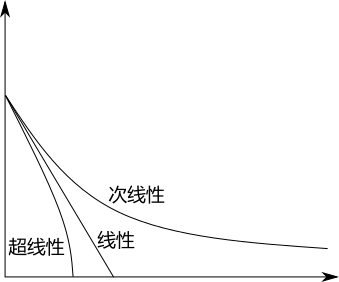
\includegraphics[width=0.3\linewidth]{fig/linear.png}
    \caption*{不同收敛速度}
\end{figure}

\begin{example}
\[f_0(\vx)=\frac{1}{2}\norm{A\vx-\vb}_2^2\]
\end{example}
\begin{analysis}
    \[\iter{\vx}{0}\to\iter{\vx}{1}\]
    \[\iter{\vx}{1}=\iter{\vx}{0}-\alpha(\iter{\vx}{0}-\vb)=\vb\]
\end{analysis}

条件数糟糕的病态矩阵收敛速度是非常糟糕的,会出现zig-zag的情况,如下面的矩阵
\[A=\bmat{1 & 0\\ 0 & 10^{-4}}\]
可以通过预处理(precondition)来解决条件数糟糕的问题

\subsubsection{收敛性分析}
$f_0(\vx)$,Lipschitz连续梯度($L$),强凸($\mu$),考虑\textbf{函数值收敛性}
\[\begin{aligned}
    \tilde{f}_0(\iter{\alpha}{k})&=f_0(\iter{\vx}{k+1})=f_0(\iter{\vx}{k}-\iter{\alpha}{k}\nabla f_0(\iter{\vx}{k}))\\
    &\leq f_0(\iter{\vx}{k})+\lrang{\nabla f_0(\iter{\vx}{k}),-\iter{\alpha}{k}\nabla f_0(\iter{\vx}{k})}+\frac{L}{2}\norm{-\iter{\alpha}{k}\nabla f_0(\iter{\vx}{k})}^2\\
    &=f_0(\iter{\vx}{k})+\frac{L(\iter{\alpha}{k})^2-2\iter{\alpha}{k}}{2}\norm{\nabla f_0(\iter{\vx}{k})}^2
\end{aligned}\]

\begin{itemize}
\item $\iter{\alpha}{k}=\iter{\alpha}{k}_{exact}$精确线搜索
\[\begin{aligned}
    &\tilde{f}_0(\iter{\alpha}{k}_{exact})\leq\tilde{f}_0\lrp{\frac{1}{L}}=f_0(\iter{\vx}{k})-\frac{1}{2L}\norm{\nabla f_0(\iter{\vx}{k})}^2\\
    \implies&\tilde{f}_0(\iter{\alpha}{k}_{exact})-f_0(\iter{\vx}{k})-f_0(\vx^\star)-\frac{1}{2L}\norm{\nabla f_0(\iter{\vx}{k})}^2
    \leq \lrp{1-\frac{\mu}{L}}(f_0(\iter{\vx}{k})+f_0(\vx^\star))
\end{aligned}\]
\[\begin{aligned}
    f_0(\vx^\star)&\geq f_0(\iter{\vx}{k})+\lrang{\nabla f_0(\iter{\vx}{k}),\vx^\star-\iter{\vx}{k}}+\frac{\mu}{2}\norm{\iter{\vx}{k}-\vx^\star}^2\\
    &\geq f_0(\iter{\vx}{k})-\frac{\mu}{2}\norm{\iter{\vx}{k}-\vx^\star}^2-\frac{1}{2\mu}\norm{\nabla f_0(\iter{\vx}{k})}^2+\frac{\mu}{2}\norm{\iter{\vx}{k}-\vx^\star}^2\qquad ab\geq-\frac{\mu}{2}a^2-\frac{1}{2\mu}b^2\\
    &= f_0(\iter{\vx}{k})-\frac{1}{2\mu}\norm{\nabla f_0(\iter{\vx}{k})}^2
\end{aligned}\]
\[f_0(\iter{\vx}{k})-f_0(\vx^\star)\leq\frac{1}{2\mu}\norm{\nabla f_0(\iter{\vx}{k})}^2\]

\item Armijo Rule
\[\tilde{f}_0(\iter{\alpha}{k})=f_0(\iter{\vx}{k+1})\leq f_0(\iter{\vx}{k})+\frac{L(\iter{\alpha}{k})^2-2\iter{\alpha}{k}}{2}\norm{\nabla f_0(\iter{\vx}{k})}^2\]
\[\tilde{f}_0(\iter{\alpha}{k})=f_0(\iter{\vx}{k+1})\leq f_0(\iter{\vx}{k})-\nabla\iter{\alpha}{k}\norm{\nabla f_0(\iter{\vx}{k})}^2\]
首先说明,若$0\leq\iter{\alpha}{k}\leq\frac{1}{L}$时,
\[\tilde{f}_0(\iter{\alpha}{k})\leq f_0(\iter{\vx}{k})-\gamma\iter{\alpha}{k}\norm{\nabla f_0(\iter{\vx}{k})}^2\]
当$\iter{\alpha}{k}\in[0,\frac{1}{2}]$时,
\[-\iter{\alpha}{k}+\frac{L}{2}(\iter{\alpha}{k})^2\leq -\frac{\iter{\alpha}{k}}{2}\iff \frac{L}{2}(\iter{\alpha}{k})^2\leq\frac{\iter{\alpha}{k}}{2}\iff L\cdot\iter{\alpha}{k}\leq 1\]
\[\begin{aligned}
    f_0(\iter{\vx}{k+1})&\leq f_0(\iter{\vx}{k})+\frac{L(\iter{\alpha}{k})^2-2\iter{\alpha}{k}}{2}\norm{\nabla f_0(\iter{\vx}{k})}^2\\
    &\leq f_0(\iter{\vx}{k})-\frac{\iter{\alpha}{k}}{2}\norm{\nabla f_0(\iter{\vx}{k})}^2\\
    &\leq f_0(\iter{\vx}{k})-\gamma\iter{\alpha}{k}\norm{\nabla f_0(\iter{\vx}{k})}^2
\end{aligned}\]
\[\begin{aligned}
    &f_0(\iter{\vx}{k+1})\leq f_0(\iter{\vx}{k})-\min\lrb{\gamma\alpha_{\max},\frac{\gamma\beta}{L}}\norm{\nabla f_0(\iter{\vx}{k})}^2\\
    \implies& f_0(\iter{\vx}{k+1})-f_0(\vx^\star)\leq\lrp{1-\min\lrb{2\mu\gamma\alpha_{\max},\frac{2\mu\gamma\beta}{L}}}(f_0(\iter{\vx}{k})-f_0(\vx^\star))
\end{aligned}\]
\end{itemize}

\subsubsection{梯度下降法的解释}
\begin{itemize}
\item 解释一
\[\iter{\vx}{k+1}=\iter{\vx}{k}-\iter{\alpha}{k}\nabla f_0(\iter{\vx}{k})\]
将$f_0$在$\iter{\vx}{k}$处进行一阶Taylor展开
\[f_0(\vx)\approx f_0(\iter{\vx}{k})+\lrang{\nabla f_0(\iter{\vx}{k}),\vx-\iter{\vx}{k}}+\frac{1}{2\iter{\alpha}{k}}\norm{\vx-\iter{\vx}{k}}^2\]
求梯度
\[\begin{aligned}
    &\nabla f_0(\iter{\vx}{k})+\frac{1}{\iter{\alpha}{k}}(\vx-\iter{\vx}{k})=0\\
    \implies &\iter{\alpha}{k}\nabla f_0(\iter{\vx}{k})+\vx-\iter{\vx}{k}=0\\
    \implies &\vx=\iter{\vx}{k}-\iter{\alpha}{k}\nabla f_0(\iter{\vx}{k})
\end{aligned}\]

\item 解释二
\[f_0(\iter{\vx}{k}+\vv)\approx f_0(\iter{\vx}{k})+\lrang{\nabla f_0(\iter{\vx}{k}),\vv}\]
\[\iter{\vd}{k}=\argmin_\vv\{\lrang{\nabla f_0(\iter{\vx}{k}),\vv}\mid \norm{\vv}=1\}\]
若采用2-范数,可得标准化的负梯度方向(normalized negative gradient)
\[\iter{\vd}{k}=\frac{-\nabla f_0(\iter{\vx}{k})}{\norm{\nabla f_0(\iter{\vx}{k})}_2}\]
通过改变不同的范数,有不同的特性
\end{itemize}

进而有\textbf{坐标下降法/交替极小化}(coordinate descent/alternating direction)
\[\iter{\vd}{k}=\ve_{k \mod n}\]
注意,这里$\vx\in\rn$,$n \mod n = n$


\subsection{非光滑优化问题}
\subsubsection{次梯度法}
同样考虑$f_0$连续,凸,不可微
\[\min\;f_0(\vx)\]
梯度\textbf{下降}法$\to$次梯度(subgradient)法\footnote{如果激活函数为非光滑的(如ReLU),那么出来的函数也是非光滑的,就要用次梯度}
\begin{definition}[次梯度]
若$g_0(\vx)\in\partial f_0(\vx)$(注意凹函数则对应的是supgradient)为$f_0(\vx)$的一个次梯度,则
\[\forall \vy:\;f_0(\vy)\geq f_0(\vx)+\lrang{g_0(\vx),\vy-\vx}\]
即过该点的直线都要在整条曲线的下方,则该直线的斜率范围为次梯度取值
\end{definition}
如$f(\vx)=|\vx|$在零点处次梯度为$[-1,1]$。

次梯度法迭代格式如下
\[\iter{\vx}{k+1}=\iter{\vx}{k}-\iter{\alpha}{k}g_0(\iter{\vx}{k})\]
只要有$0\in\partial f_0(\vx_0)$就有最优解$\vx=\vx_0$

对于梯度法来说,关键在于选择步长
\begin{itemize}
    \item 固定步长$\iter{\alpha}{k}=\alpha$
    \item 不可加但平方可加,如$\frac{1}{k}$
    \[\sum_{k=0}^\infty \iter{\alpha}{k}=\infty\qquad\sum_{k=0}^\infty(\iter{\alpha}{k})^2<\infty\]
    \item 不可加递减,如$\frac{1}{\sqrt{k}}$
    \[\sum_{k=0}^\infty\iter{\alpha}{k}=0\qquad\lim_{k\to\infty}\iter{\alpha}{k}\to 0\]
\end{itemize}

考虑次梯度法的\textbf{收敛速度}
\[\inf_{i=0,\ldots,k}(f_0(\iter{\vx}{i})-f_0(\vx^\star))\]
% \[\iter{\bar{\vx}}{k}:=\frac{\sum_{i=0}^k\iter{\alpha}{i}\iter{\vx}{i}}{\sum_{i=0}^k\iter{\alpha}{i}}\]
% \[f_0(\iter{\bar{\vx}}{k})-f_0(\vx^\star)\]

假设函数Lipschitz连续
\[\exists G>0,\forall \vx,\vy:\;\norm{f_0(\vx)-f_0(\vy)}\leq G\norm{\vx-\vy}\]
对任意最优解$\vx^\star$,有
\[\begin{aligned}
    &\norm{\iter{\vx}{k+1}-\vx^\star}^2=\norm{\iter{\vx}{k}-\iter{\alpha}{k}g_0(\iter{\vx}{k})-\vx^\star}^2\\
    =&\norm{\iter{\vx}{k}-\vx^\star}^2-2\lrang{\iter{\alpha}{k}g_0(\iter{\vx}{k}),\iter{\vx}{k}-\vx^\star}+(\iter{\alpha}{k})^2\norm{g_0(\iter{\vx}{k})}^2\qquad\mbox{拆平方}\\
    \leq& \norm{\iter{\vx}{k}-\vx^\star}^2-2(\iter{\alpha}{k})^2(f_0(\iter{\vx}{k})-f_0(\vx^\star))+(\iter{\alpha}{k})^2 G^2\qquad\mbox{多次迭代}\\
    \implies& \norm{\iter{\vx}{k+1}-\vx^\star}^2\leq \norm{\iter{\vx}{0}-\vx^\star}^2-2\sum_{i=0}^k\iter{\alpha}{i}(f_0(\iter{\vx}{i})-f_0(\vx^\star))+\sum_{i=0}^k(\iter{\alpha}{i})^2 G^2\\
    \implies& 2\sum_{i=0}^k\iter{\alpha}{i}(f_0(\iter{\vx}{i})-f_0(\vx^\star))\leq \norm{\iter{\vx}{0}-\vx^\star}^2+\sum_{i=0}^k(\iter{\alpha}{i})^2G^2\\
    &\sum_{i=0}^k\iter{\alpha}{i}(f_0(\iter{\vx}{i})-f_0(\vx^\star))\geq\lrp{\sum_{i=0}^k\iter{\alpha}{i}}\inf_{i=0,\ldots,k}(f_0(\iter{\vx}{i})-f_0(\vx^\star))\\
    \implies&\inf_{i=0,\ldots,k}(f_0(\iter{\vx}{i})-f_0(\vx^\star))\leq\frac{\disp\norm{\iter{\vx}{0}-\vx^\star}^2+G^2\sum_{i=0}^k(\iter{\alpha}{i})^2}{\disp 2\sum_{i=0}^k\iter{\alpha}{i}}
\end{aligned}\]

这是一个紧的界
\begin{itemize}
    \item 固定步长得到上界$\frac{G^2\alpha}{2}$,以$f(x)=|x|$为例
    \item 不可加平方可加一定收敛,若步长为$\frac{1}{k}$,收敛速度为$\frac{1}{\log k}$(幂级数积分取上下界$\sum_{i=0}^k\frac{1}{i}=O(\log k)$)
    \item 不可加平方不可加同样收敛,若步长为$\frac{1}{\sqrt{k}}$,收敛速度为$O\lrp{\frac{\log k}{\sqrt{k}}}$,可以证明在该假设下该收敛速度最优
\end{itemize}

\[\lim_{k\to\infty}\inf_{i=0,\ldots,k}\lrp{f_0(\iter{\vx}{i})-f_0(\vx^\star)}=0\]
\[\forall \eps>0,\exists N_1\in\zz, \forall i>N_1:\;\iter{\alpha}{i}\leq\frac{\eps}{G^2}\]
\[\exists N_2\in\zz,\forall k>N_2:\;\sum_{i=0}^k\iter{\alpha}{i}\geq\frac{1}{\eps}\lrp{\norm{\iter{\vx}{0}-\vx^\star}^2+G^2\sum_{i=0}^{N_1}(\iter{\alpha}{i})^2}\]
令$N=\max\{N_1,N_2\},\forall k>N$
\[\dfrac{\disp \norm{\iter{\vx}{0}-\vx^\star}^2+G^2\sum_{i=0}^{N_1}(\iter{\alpha}{i})^2}{\disp 2\sum_{i=0}^k\iter{\alpha}{i}}+\dfrac{\disp \norm{\iter{\vx}{0}-\vx^\star}^2+G^2\sum_{i=N_1+1}^{k}(\iter{\alpha}{i})^2}{\disp 2\sum_{i=0}^{N_1}\iter{\alpha}{i}+2\sum_{i=N_1+1}^{k}\iter{\alpha}{i}}\leq\frac{\eps}{2}+\frac{\eps}{2}=\eps\]
\[\text{第二项}\leq\dfrac{\disp G^2\sum_{i=N_1+1}^k\iter{\alpha}{i}\frac{\eps}{G^2}}{\disp 2\sum_{i=0}^{N_1}\iter{\alpha}{i}+2\sum_{i=N_1+1}^{k}\iter{\alpha}{i}}\leq\frac{\eps}{2}\]
实际上这个假设一般情况下不成立,但是我们只需保证在优化路径上成立即可,也有设置$\vx$有界的

\subsubsection{邻近点梯度法(proximal gradient method)}
考虑有\textbf{结构},不可微的函数
\[\min f_0(\vx)=s(\vx)+r(\vx)\]
\begin{itemize}
    \item $s$: smooth,可微,易求导
    \item $r$: regularization,不可微,易求邻近点投影
\end{itemize}

\begin{definition}[邻近点投影(proximal mapping)]
    函数$r$和平衡参数$\alpha$的近端算子
\[\opprox_r \hat{\vx}=\argmin_\vx \lrp{r(\vx)+\frac{1}{2\alpha}\norm{\vx-\hat{\vx}}_2^2}\]
\begin{figure}[H]
    \centering
    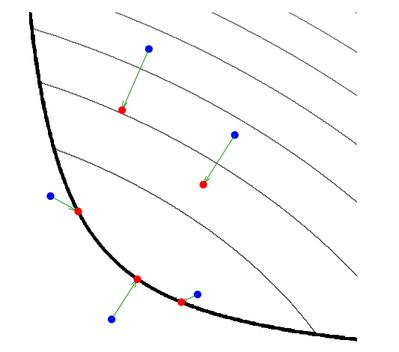
\includegraphics[width=0.4\linewidth]{fig/prox.jpg}
\end{figure}
注:邻近点/近端投影字面上理解即对点$\hat{\vx}$关于$r$下降方向的邻近点。
如上图,黑细线为$r$的水平集,黑粗线为定义域边界,蓝色点为$\hat{\vx}$,红色为作用该算子后的点,这些点都统一朝着函数最小的方法前进\footnote{详细见\url{https://zhuanlan.zhihu.com/p/37444622}}。
\end{definition}
邻近点梯度法迭代格式如下
\[\begin{cases}
    \iter{\vx}{k+\frac{1}{2}}=\iter{\vx}{k}-\iter{\alpha}{k}\nabla s(\iter{\vx}{k})\\
    \iter{\vx}{k+1}=\opprox_{r}\iter{\vx}{k+\frac{1}{2}}=\argmin_\vx\lrp{r(\vx)+\frac{1}{2\alpha}\norm{\vx-\iter{\vx}{k+\frac{1}{2}}}_2^2}
\end{cases}\]

\begin{example}[LASSO]
    \[f(\vx)=\frac{1}{2}\norm{A\vx-\vb}_2^2+p\norm{\vx}_1\]
\end{example}
\begin{analysis}
    设
    \[\begin{cases}
    s(\vx):=\dfrac{1}{2}\norm{A\vx-\vb}_2^2\\
    r(\vx):=p\norm{\vx}_1
    \end{cases}\]
    其中,$A\in\rr^{m\times n}$,$\vx\in\rr^n$,$\vb,\ve\in\rr^m$(在本题中$m=50,n=100$),$s(\vx)$为光滑函数,$r(\vx)$为非光滑函数,则原式
    \[f(\vx)=s(\vx)+r(\vx)\]
    先求$r(\vx)$的邻近点投影
    \[\opprox \hat{\vx}=\argmin_\vx\lrp{p\norm{\vx}_1+\frac{1}{2\alpha}\norm{\vx-\hat{\vx}}_2^2}\]
    对上式右侧展开有
    \[\argmin_\vx\lrp{p\sum_{i=1}^n|x_i|+\frac{1}{2\alpha}\sum_{i=1}^n(x_i-\hat{x}_i)^2}\]
    注意到上式对于下标$i$相互独立,故要求上式的最小值,等价于对每一个下标$i$求最小值后求和,即
    \[\argmin_{x_i}\lrp{p|x_i|+\frac{1}{2\alpha}(x_i-\hat{x}_i)^2},\;\forall i\]
    由不可微函数的极值判断条件有
    \[0\in\lrp{\partial_{x_i}p|x_i|+\frac{1}{\alpha}(x_i-\hat{x}_i)},\;\forall i\]
    对每一个$x_i$进行分类讨论
    \begin{itemize}
        \item 若$x_i>0$,则$|x_i|$对于$x_i$可微,即$\partial_{x_i}|x_i|=1$,有
        \[p+\frac{1}{\alpha}(x_i-\hat{x}_i)=0\]
        整理得
        \[x_i=\hat{x}_i-\alpha p\]
        由于$x_i>0$,故$\hat{x}_i-\alpha p>0$,即$\hat{x}_i>\alpha p$
        \item 若$x_i<0$,则$|x_i|$对于$x_i$可微,即$\partial_{x_i}|x_i|=-1$,有
        \[-p+\frac{1}{\alpha}(x_i-\hat{x}_i)=0\]
        整理得
        \[x_i=\hat{x}_i+\alpha p\]
        由于$x_i<0$,故$\hat{x}_i+\alpha p<0$,即$\hat{x}_i<-\alpha p$
        \item 若$x_i=0$,则$|x_i|$对于$x_i$不可微,需要求次梯度,$\partial_{x_i}|x_i|=[-1,1]$,即
        \[0\in\left[-p-\frac{\hat{x}_i}{\alpha},p-\frac{\hat{x}_i}{\alpha}\right]\]
        那么,需要满足
        \[\begin{cases}
        p-\dfrac{\hat{x}_i}{\alpha}\geq 0\\
        -p-\dfrac{\hat{x}_i}{\alpha}\leq 0
        \end{cases}\]
        推得
        \[\hat{x}_i\in[-\alpha p,\alpha p]\]
    \end{itemize}
    综上,有
    \[x_i=\begin{cases}
    \hat{x}_i+\alpha p & \hat{x}_i<-\alpha p\\
    0 & \hat{x}_i\in[-\alpha p,\alpha p]\\
    \hat{x}_i-\alpha p & \hat{x}_i>\alpha p
    \end{cases}\]
    可以得到下图的软门限(soft-thresholding)曲线
    \begin{figure}[H]
    \centering
    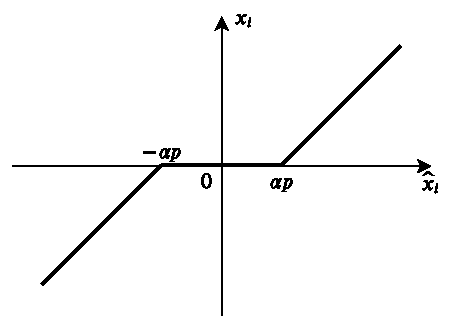
\includegraphics[width=0.4\linewidth]{fig/soft-thresholding.pdf}
    \end{figure}

    进一步,得到邻近点梯度下降法的迭代式如下
    \[\begin{cases}
    \iter{\vx}{k+\frac{1}{2}}=\iter{\vx}{k}-\alpha\nabla s(\iter{\vx}{k})=\iter{\vx}{k}-\alpha A^T(A\iter{\vx}{k}-\vb)\\
    \iter{\vx}{k+1}=\opprox \iter{\vx}{k+\frac{1}{2}}=\argmin_\vx\lrp{p\norm{\vx}_1+\dfrac{1}{2\alpha}\norm{\vx-\iter{\vx}{k+\frac{1}{2}}}_2^2}
    \end{cases}\]
    其中,$\iter{x}{k+\frac{1}{2}}$可直接计算,$\iter{x}{k+1}$的显式解可由软门限求得。\\
    此算法即迭代阈值收缩(Iterative shrinkage-thresholding algorithm,ISTA)算法
\end{analysis}

\begin{example}[盒限制(box constrained)优化问题]
\[f_0(\vx)=s(\vx)+\sum_{i=1}^nI(x_i\in[l_i,u_i])\]
\end{example}
\begin{analysis}
    构造邻近点投影
\begin{argmini*}
    {}{\frac{1}{2\alpha}\norm{\vx-\hat{\vx}}^2}{}{}
    \addConstraint{x_i\in[l_i,u_i]}{,\forall i}
\end{argmini*}
如果有约束$\vx\in\sC$
\[\begin{cases}
    \iter{\vx}{k+\frac{1}{2}}=\iter{\vx}{k}-\alpha\nabla S(\iter{\vx}{k})\\
    \iter{\vx}{k+1}=\argmin_\vx \lrp{I_\sC(\iter{\vx}{k+\frac{1}{2}})+\frac{1}{2\alpha}\norm{\vx-\iter{\vx}{k+\frac{1}{2}}}^2}=\argmin_\vx\frac{1}{2\alpha}\norm{\vx-\iter{\vx}{k+\frac{1}{2}}}^2,\vx\in\sC
\end{cases}\]
相当于做投影,故称投影梯度法
    \[\begin{aligned}
        0&\in\partial r(\iter{\vx}{k+1})+\frac{1}{\alpha}(\iter{\vx}{k+1}-\iter{\vx}{k+\frac{1}{2}})\\
        0&=\partial r(\iter{\vx}{k+1})+\frac{1}{\alpha}(\iter{\vx}{k+1}-\iter{\vx}{k}+\alpha\nabla S(\iter{\vx}{k}))\\
        \iter{\vx}{k+1}&=\iter{\vx}{k}-\alpha\nabla S(\iter{\vx}{k})-\alpha\partial r(\iter{\vx}{k+1})
    \end{aligned}\]
\end{analysis}

数值计算:显式方法(次梯度法)$\to$隐式方法(邻近点梯度法---需要先知道下一步信息,但是这是可以做的,因为有邻近点)

* 邻近点投影法的收敛性能与梯度下降法类似

\begin{example}[矩阵补全]
    $Y\in\rr^{m\times n},\{Y_{ij},(i,j)\in\Omega\}$
    \[\min_B\lrp{\frac{1}{2}\sum_{(i,j)\in\Omega}(Y_{ij}-B_{ij})^2+\lambda\oprank(B)}\]
\end{example}
\begin{analysis}
    同LASSO,由于矩阵的秩(奇异值向量0-范数)不好求,改为矩阵的和范数$\norm{\cdot}$(奇异值向量1-范数),即
    \[\min_B\lrp{\frac{1}{2}\sum_{(i,j)\in\Omega}(Y_{ij}-B_{ij})^2+\lambda\norm{B}_\star}\]
    其中,
    \[\norm{B}_\star:=\sum_{i=1}^n\sigma_i(B)\]
    \[\min\lrp{\frac{1}{2}\norm{P_\Omega(B-Y)}_F^2+\lambda\norm{B}_\star}\]
    若原矩阵中该项不存在,$P_\Omega$为$0$;存在的话则保持不变
    \[\nabla B\lrp{\frac{1}{2}\norm{P_\Omega}(B-Y)_F^2}=P_\Omega(B-Y)\]
    对$B$做奇异值分解,$U$为酉矩阵
    \[\partial\norm{B}_\star=\{UDV^\T, B=U\Sigma V^\T, d=\partial\norm{\sigma}_1\}\]
    邻近点梯度迭代格式为
    \[\begin{cases}
        \iter{B}{k+\frac{1}{2}}=B^k-\alpha P_\Omega(B^k-Y)\\
        \iter{B}{k+1}=\arg\min_B\lrp{\lambda\norm{B}_\star+\frac{1}{2\alpha}\norm{B-\iter{B}{k+\frac{1}{2}}}_F^2}
    \end{cases}\]
    求次梯度
    \[0\in\lambda\partial\norm{B}_\star+\frac{1}{\alpha}(B-\iter{B}{k+\frac{1}{2}})\]
    \[0\in\lrs{\lambda UDV^\T+\frac{1}{\alpha}(B-\iter{B}{k+\frac{1}{2}})},\;B=U\Sigma V^\T,\;D=\partial\norm{\sigma}_1\]
    \[0\in\lrb{\lambda UDV^\T +\frac{1}{\alpha}(V\Sigma V^\T-\iter{B}{k+\frac{1}{2}})}\]
    \[\exists V:\;0=\alpha\lambda UDV^\T+V\Sigma V^\T-\iter{B}{k+\frac{1}{2}}\]
    \[\iter{B}{k+\frac{1}{2}}=U(\alpha\lambda D+\Sigma)V^\T\]
    对$\iter{B}{k+\frac{1}{2}}$进行奇异值分解
    \[\iter{B}{k+\frac{1}{2}}=U\iter{\Sigma}{k+\frac{1}{2}}V\]
    \[T_i=\alpha\lambda d_i+\sigma_i\]
    若$\sigma_i\ne 0\implies \tau_i=\alpha\lambda+\sigma_i$\\
    若$\sigma_i=0\implies \tau_i\in[-\alpha\lambda+\sigma_i,\alpha\lambda+\sigma_i]$\\
    \[\begin{cases}
        \sigma_i=\tau_i-\alpha\lambda & \tau_i>\alpha\lambda\\
        \sigma_i=0 & \tau_i\leq\alpha\lambda
    \end{cases}\]
    该算法称为矩阵软门限算法
\end{analysis}

\subsection{二阶优化方法}
\subsubsection{牛顿法}
牛顿法(Newton's method):要求$f_0(\vx)$二阶可微,强凸,考虑不同方向,用Taylor展开有
\[\begin{aligned}
    \min f_0(\iter{\vx}{k}+\vd)&\approx\min_{\vd}\lrp{f_0(\iter{\vx}{k})+\lrang{\nabla f_0(\iter{\vx}{k}),\vd}}\\
    &\approx\min_\vd \lrp{f_0(\iter{\vx}{k})+\nabla f_0(\iter{\vx}{k})^\T\vd+\frac{1}{2}\vd^\T \nabla^2f_0(\iter{\vx}{k})\vd}
\end{aligned}\]
对$\vd$求梯度有
\[\begin{aligned}
    \qquad&\nabla f_0(\iter{\vx}{k})+\nabla^2f_0(\iter{\vx}{k})\vd=0\\
    \implies& \vd=-(\nabla^2f_0(\iter{\vx}{k}))^{-1}\nabla f_0(\iter{\vx}{k})\to\text{牛顿方向}
\end{aligned}\]
得到牛顿法的迭代格式如下
\[\iter{\vx}{k+1}=\iter{\vx}{k}-\iter{\alpha}{k}(\nabla^2 f_0(\iter{\vx}{k}))^{-1}\nabla f_0(\iter{\vx}{k})\]
其中$\iter{\alpha}{k}$为搜索步长。

看下降方向只要看其与负梯度方向是否小于90度
\[\begin{aligned}
    \qquad& \lrang{-\nabla f_0(\iter{\vx}{k}),-(\nabla^2 f_0(\iter{\vx}{k}))^{-1}\nabla f_0(\iter{\vx}{k})}\\
    =&\nabla^\T f_0(\iter{\vx}{k})(\nabla^2 f_0(\iter{\vx}{k}))^{-1}\nabla f_0(\iter{\vx}{k})
\end{aligned}\]

假设$\nabla^2f_0(\vx)$Lipschitz连续
\begin{itemize}
    \item 若$\norm{\nabla f_0(\iter{\vx}{k})}_2>\eta$,阻尼(damped)牛顿段\\
用Armijo Rule算步长,$\exists\gamma>0$,$f_0(\iter{\vx}{k+1})-f_0(\iter{\vx}{k})\leq-\gamma$
    \item 若$\norm{\nabla f_0(\iter{\vx}{k})}_2\leq\eta$,纯牛顿段\\
$\alpha=1,f_0(\iter{\vx}{k+1})-f_0(\vx^\star)\leq\Delta(\frac{1}{2})^{2^k},\exists\Delta>0$,超线性收敛
\end{itemize}
多了二阶信息,往最优解跑的速度会越来越快

\begin{example}
    \begin{mini*}
        {}{\frac{1}{2}\vx^\T P\vx+\vq^\T \vr+c}{}{}
        \addConstraint{P}{\succ 0}
    \end{mini*}
\end{example}
\begin{analysis}
    对于二阶强凸问题,只需1步到达最优解;但用梯度下降法,与条件数相关
\end{analysis}
与Newton-Raphson算法的联系:将其扩展至高维的凸问题
\[\iter{\vx}{k+1}=\iter{\vx}{k}-\frac{g(\iter{\vx}{k})}{g'(\iter{\vx}{k})}\]

\subsubsection{拟牛顿法}
拟牛顿法(quasi-Newton):希望像一阶算法一样好算,又像二阶算法一样收敛快
\begin{enumerate}
    \item 构造$(\nabla^2f_0(\iter{\vx}{k}))^{-1}$的近似矩阵$\iter{G}{k}$(直接的想法)
    \item 构造$\nabla^2f_0(\iter{\vx}{k})$的近似矩阵$\iter{B}{k}$,且容易求逆
\end{enumerate}
在$\vx=\iter{\vx}{k+1}$点处做Taylor展开
\[\begin{aligned}
    \qquad & f_0(\vx)\approx f_0(\iter{\vx}{k+1})+\lrang{\nabla f_0(\iter{\vx}{k+1}),\vx-\iter{\vx}{k+1}}+\frac{1}{2}(\vx-\iter{\vx}{k+1})^\T\nabla^2 f_0(\iter{\vx}{k+1})(\vx-\iter{\vx}{k+1})\\
    \implies&\nabla f_0(\vx)\approx\nabla f_0(\iter{\vx}{k+1})+\nabla^2 f_0(\iter{\vx}{k+1})(\vx-\iter{\vx}{k+1})\\
    \implies&\nabla f_0(\iter{\vx}{k})\approx\nabla f_0(\iter{\vx}{k+1})+\nabla^2 f_0(\iter{\vx}{k+1})(\iter{\vx}{k}-\iter{\vx}{k+1})\\
    \implies&\nabla f_0(\iter{\vx}{k})-\nabla f_0(\iter{\vx}{k+1})\approx\nabla^2 f_0(\iter{\vx}{k+1})(\iter{\vx}{k}-\iter{\vx}{k+1})
\end{aligned}\]
\[\begin{cases}
    \iter{\vq}{k}=\nabla f_0(\iter{\vx}{k+1})-\nabla f_0(\iter{\vx}{k})\\
    \iter{\vp}{k}=\iter{\vx}{k+1}-\iter{\vx}{k}
\end{cases}\implies
\begin{cases}
    \iter{\vq}{k}=\iter{B}{k+1}\iter{\vp}{k}\\
    \iter{\vp}{k}=\iter{G}{k+1}\iter{\vq}{k}
\end{cases}\]
\begin{enumerate}
\item 近似$\iter{G}{k}$
\[\iter{G}{k+1}=\iter{G}{k}+\Delta\iter{G}{k}\]
\begin{itemize}
    \item [a.]秩1校正(希望$G$中不要有太多元素,故用低秩矩阵做近似)
    \[\Delta\iter{G}{k}=\iter{\alpha}{k}\iter{\vz}{k}(\iter{\vz}{k})^\T\]
    \[\iter{\vp}{k}=\iter{G}{k+1}\iter{\vq}{k}=\iter{G}{k}\iter{\vq}{k}+\iter{\alpha}{k}\iter{\vz}{k}(\iter{\vz}{k})^\T\iter{\vq}{k}\]
    \[\implies\Delta\iter{G}{k}=\frac{(\iter{\vp}{k}-\iter{G}{k}\iter{\vq}{k})(\iter{\vp}{k}-\iter{G}{k}\iter{\vq}{k})^\T}{(\iter{\vq}{k})^\T(\iter{\vp}{k}-\iter{G}{k}\iter{\vq}{k})}\]
    稳定性很有问题,分母接近0的时候,越接近最优解越不稳定
    \item [b.]秩2校正(Dandon-Fletcher-Power, DFP)
    \[\Delta\iter{G}{k}=\frac{\iter{\vp}{k}(\iter{\vp}{k})^\T}{(\iter{\vp}{k})^\T\iter{\vq}{k}}-\frac{\iter{G}{k}\iter{\vq}{k}(\iter{\vq}{k})^\T\iter{G}{k}}{(\iter{\vq}{k})^\T\iter{G}{k}\iter{\vq}{k}}\]
    前后项都为秩1矩阵,数值稳定性强
\end{itemize}
\item 近似$\iter{B}{k}$(Broyden-Fletcher-Goldfarb-Shermo, BFGS)
\[\iter{B}{k+1}=\iter{B}{k}+\frac{\iter{\vq}{k}(\iter{\vq}{k})^\T}{(\iter{\vq}{k})^\T\iter{\vp}{k}}-\frac{\iter{B}{k}\iter{\vp}{k}(\iter{\vp}{k})^\T\iter{B}{k}}{(\iter{\vp}{k})^\T\iter{B}{k}\iter{\vp}{k}}\]
\end{enumerate}
\begin{itemize}
    \item 拟牛顿法以后可能很有用,因为结合一二阶优化优点
    \item 找核心问题(Hessian矩阵难算),然后就去解决
    \item 用\textbf{结构信息},都对结构进行限制(一股脑就用Adam优化器,这是不对的,要分析问题结构)
\end{itemize}

有限内存(limited memory)---LM-BFGS

\subsection{约束满足的牛顿法}
考虑有约束优化问题
\begin{mini*}
    {}{f_0(\vx)}{}{}
    \addConstraint{A \vx}{=\vb}
\end{mini*}

本质上都是在考虑它的KKT条件
\[\begin{cases}
    A \vx^\star=\vb\\
    \nabla f_0(\vx^\star)+A^\T \vv^\star=0
\end{cases}\]
\begin{example}
\begin{mini*}
    {}{\frac{1}{2}\vx^\T P\vx+\vq^\T \vx+r,P\succeq 0}{}{}
    \addConstraint{A\vx}{=\vb}
\end{mini*}
\end{example}
\begin{analysis}
等价于KKT条件
\[\begin{cases}
    A \vx^\star=\vb\\
    P \vx^\star+\vq+A^\T \vv^\star=0
\end{cases}\]
等价于
\[\bmat{P & A^\T\\A & \vzero}\bmat{\vx^\star \\\vv^\star}=\bmat{-\vq\\\vb}\]
\end{analysis}

若方程组非线性,那就做一个线性化,近似等价于二阶近似的Taylor展开
\begin{argmini*}
{\vd}{f_0(\iter{\vx}{k}+\vd)=\iter{\vd}{k}\approx f_0(\iter{\vx}{k})+\lrang{\nabla f_0(\iter{\vx}{k}),\vd}+\frac{1}{2}\vd^\T\nabla^2 f_0(\iter{\vx}{k})\vd=\iter{\vd}{k}}{}{}
\addConstraint{A(\iter{\vx}{k}+\vd)}{=\vb}
\end{argmini*}

写出问题关于$\vd$的KKT条件,可得约束满足牛顿法的迭代格式
\[\bmat{\nabla^2 f_0(\iter{\vx}{k}) & A^\T\\ A & \vzero^\T}\bmat{\iter{\vd}{k}\\\iter{\vv}{k}}=\bmat{-\nabla f_0(\iter{\vx}{k})\\\vb-A\iter{\vx}{k}}\]

若$\iter{\vx}{0}$可行,$A\iter{\vx}{0}=\vb$,之后的$\iter{\vx}{k+1}=\iter{\vx}{k}+\iter{\alpha}{k}\iter{\vd}{k}$也可行。

\subsection{原对偶方法}
\subsubsection{拉格朗日乘子法/对偶分解法}
\[L(\vx,\vv)=f_0(\vx)+\lrang{\vv,A\vx-\vb}\]
更新原变量和对偶变量,迭代格式如下
\[\begin{cases}
    \iter{\vx}{k+1}=\argmin_\vx L(\vx,\iter{\vv}{k})\\
    \iter{\vv}{k+1}=\iter{\vv}{k}+\iter{\alpha}{k}(A\iter{\vx}{k+1}-\vb)
\end{cases}\]
$\iter{\alpha}{k}$可以是固定步长,也可以是递减步长

即为\textbf{找鞍点},$\vx$方向上找最小值,本来$\vv$方向上要找最大值,但容易到正无穷。因此换种方法$\iter{\vv}{k}$做一个保守的计算,每一步都走一个很小的步长。
实际上$A\vx-\vb$即为$\nabla_\vv L(\vx,\vv)$,故属于梯度上升法。

\begin{example}
    \begin{mini*}
        {}{\frac{1}{2}x^2}{}{}
        \addConstraint{x}{=1}
    \end{mini*}
\end{example}
\begin{analysis}
    \[\begin{aligned}
        L(x,v)&=\frac{1}{2}x^2+v(x-1)\\
        &=\frac{1}{2}x^2+vx-v
    \end{aligned}\]
\end{analysis}

\subsubsection{原对偶次梯度法}
$\vv$才是最关键的,只是在寻找最优$\vv$的时候顺带找到了$\vx$(收敛到$\vv^\star$的同时也找到了$\vx^\star$),考虑对偶函数
\[D(\vv)=\inf_\vx L(\vx,\vv)\]
$D(\vv)$为凹函数,关注$-D(\vv)$
\[\begin{cases}
    \iter{\vx}{k+1}=\argmin_\vx L(\vx,\iter{\vv}{k})\\
    \iter{\vv}{k+1}=\iter{\vv}{k}-\iter{\alpha}{k}(-(A\iter{\vx}{k+1}-\vb))
\end{cases}\]

若$f_0(\vx)$为凸,$\hat{\vx}=\argmin_\vx L(\vx,\hat{\vlambda})$
\[\begin{aligned}
    D(\vv)&=\inf_\vx L(\vx,\vv)\\
    &=\inf_\vx \lrp{f_0(\vx)+\lrang{\vv,A\vx+\vb}}\\
    &\leq f_0(\hat{\vx})+\lrang{\vv,A\hat{\vx}-\vb}\\
    &=f_0(\hat{\vx})+\lrang{\vlambda,A\hat{\vx}-\vb}+\lrang{\vv-\hat{\vlambda},A\hat{\vx}-\vb}\\
    &=D(\hat{\vlambda})+\lrang{\vv-\hat{\vlambda},A\hat{\vx}-\vb}\\
    -D(\vv)&\geq -D(\hat{\vlambda})+\lrang{\vv-\hat{\vlambda},-(A\hat{\vx}-\vb)}
\end{aligned}\]
进而$-(A\hat{\vx}-\vb)$为$-D(\vlambda)$在$\hat{\vlambda}$的次梯度

这个算法一般来说性能不好,在机器学习里面很多时候都被乱用,有时候可以,有时候不行。
\begin{itemize}
\item 在什么情况下它是好用的?
对偶函数是可微的,采用固定步长。
\item 对偶函数$D(\vv)$何时可微?
任何$-D(\vlambda)$都具有$-(A\hat{\vx}-\vb)$的形式,得到当$f_0(\vx)$\textbf{严格凸}时,$f_0(\vx)+\lrang{\hat{\vlambda},A\vx-\vb}$严格凸,进而$D(\vv)$可微
\end{itemize}

既然计算量出在$\iter{\vx}{k+1}$,那么想办法近似
\[\begin{cases}
    \iter{\vx}{k+1}&=\iter{\vx}{k}-\iter{\alpha}{k}\partial_\vx L(\vx,\iter{\vv}{k})\\
    \iter{\vv}{k+1}&=\iter{\vv}{k}+\iter{\alpha}{k}\partial_\vv L(\iter{\vx}{k+1},\vv)
    =\iter{\vv}{k}+\iter{\alpha}{k}(A\iter{\vx}{k+1}-\vb)\\
    &\to \iter{\vv}{k}+\iter{\alpha}{k}(A\iter{\vx}{k}-\vb)
\end{cases}\]

由于$\iter{\vv}{k+1}$需要等待$\iter{\vx}{k+1}$,将其换成下式可以不用等待;
但由于两个方向都不精确,故收敛性质糟糕。

\subsubsection{增广拉格朗日法}
增广拉格朗日法(Augumented Lagrange Method, ALM):当函数不是严格凸时,依然能得到很好的效果
\begin{mini*}
    {}{f_0(\vx)}{}{}
    \addConstraint{A\vx}{=\vb}
\end{mini*}
\[L(\vx,\vv)=f_0(\vx)+\lrang{\vv,A\vx-\vb}=f_0(\vx)+\vv^\T(A\vx-\vb)\]
增广拉格朗日函数(即在最后补充$c/2\norm{f_i(\vx)}_2^2$的正则化项)
\[L_c(\vx,\vv)=f_0(\vx)+\lrang{\vv,A\vx-\vb}+\frac{c}{2}\norm{A\vx-\vb}^2,c>0\]
增广拉格朗日函数是下面问题的拉格朗日函数
\begin{mini*}
    {}{f_0(\vx)+\frac{c}{2}\norm{A\vx-\vb}^2}{}{}
    \addConstraint{A\vx}{=\vb}
\end{mini*}
两个问题的原对偶最优解相同

设$(\vx^\star,\vv^\star)$为原问题最优解,分别有以下两个KKT条件
\[\begin{cases}
    A\vx^\star=\vb\\
    \pd{L(\vx,\vv^\star)}{\vx}\Big|_{\vx=\vx^\star}=0
\end{cases}\qquad\qquad
\begin{cases}
    A\vx^\star=\vb\\
    \pd{L_c(\vx,\vv^\star)}{\vx}\Big|_{\vx=\vx^\star}=0
\end{cases}\]
对于原问题有
\[\nabla_\vx(f_0(\vx)+\lrang{\vv^\star,A\vx-\vb})\Big|_{\vx=\vx^\star}=0\]
对于对偶问题有
\[\begin{aligned}
    \qquad&\nabla_\vx\lrp{f_0(\vx)+\lrang{\vv^\star,A\vx-\vb}+\frac{c}{2}\norm{A\vx-\vb}^2}\Big|_{\vx=\vx^\star}\\
    =&\nabla_\vx\lrp{\frac{c}{2}\norm{A\vx-\vb}^2}\Big|_{\vx=\vx^\star}\qquad\mbox{原问题最优解代入}\\
    =&cA^\T(A\vx^\star-\vb)=0
\end{aligned}\]

得到增广拉格朗日法的迭代格式
\[\begin{cases}
    \iter{\vx}{k+1}=\argmin_\vx L_c(\vx,\iter{\vv}{k})\\
    \iter{\vv}{k+1}=\iter{\vv}{k}+c(A\iter{\vx}{k+1}-\vb)
\end{cases}\]
只要原问题是凸问题,无论$c$怎么取($c$刚好就是固定步长),该算法总是可以收敛(不考虑计算精度的问题),只是收敛速度不同

% 考试必考手算原变量和对偶变量
\begin{example}
    \begin{mini*}
        {}{\frac{1}{2}x_1^2+\frac{1}{2}x_2^2}{}{}
        \addConstraint{x_1}{=1}
    \end{mini*}
\end{example}
\begin{analysis}
    \[L(\vx,v)=\frac{1}{2}x_1^2+\frac{1}{2}x_2^2+v(x_1-1)\]
    \[\pd{L(\vx,v^\star)}{\vx}\Big|_{\vx=\vx^\star}=0=\bmat{x_1+v^\star\\x_2}\]
    增广拉格朗日法
    \[L_{\iter{c}{k}}(\vx,v)=\frac{1}{2}x_1^2+\frac{1}{2}x_2^2+v(x_1-1)+\frac{\iter{c}{k}}{2}(x_1-1)^2\]
    \[\iter{\vx}{k+1}=\arg\min L_{\iter{c}{k}}(\vx,\iter{v}{k})\]
    \[\begin{cases}
        x_1+\iter{v}{k}+\iter{c}{k}(x_1-1)=0\\
        x_2=0
    \end{cases}\implies
    \iter{\vx}{k+1}=\bmat{\frac{\iter{c}{k}-\iter{v}{k}}{\iter{c}{k}+1}\\0}\]
    \[\begin{aligned}
        \iter{v}{k+1}&=\iter{v}{k}+\iter{c}{k}(\iter{x_1}{k+1}-1)\\
        &=\iter{v}{k}+\iter{c}{k}\lrp{\frac{\iter{c}{k}-\iter{v}{k}}{\iter{c}{k}+1}-1}\\
        &=\frac{\iter{v}{k}}{\iter{c}{k}+1}-\frac{\iter{c}{k}}{\iter{c}{k}+1}
    \end{aligned}\]
    \[\iter{v}{k+1}-v^\star=\iter{v}{k+1}+1=\frac{\iter{v}{k}}{\iter{c}{k}+1}+\frac{1}{\iter{c}{k}+1}=\frac{\iter{v}{k}-v^\star}{\iter{c}{k}+1}\]
    可以看出取一个固定步长,且大于零,增广拉格朗日的收敛是非常好的(线性收敛)\\
    对于特殊的一些非凸问题,增广拉格朗日也是有效的,如把问题改成
    \[\min \lrp{-\frac{1}{2}x_1^2+\frac{1}{2}x_2^2}\]
\end{analysis}

\subsubsection{交替方向乘子法}
交替方向乘子法(alternating direction method of multipliers, ADMM)同样探究\textbf{有结构}的优化问题。
\begin{mini*}
    {\vx,\vy}{f(\vx)+g(\vy)}{}{}
    \addConstraint{A\vx+B\vy}{=0}
\end{mini*}
考虑增广拉格朗日函数
\[\begin{aligned}
    L_c(\vx,\vy,\vv)&=f(\vx)+g(\vy)+\lrang{\vv,A\vx+B\vy}+\frac{c}{2}\norm{A\vx+B\vy}_2^2\\
    &=f(\vx)+g(\vy)+\frac{c}{2}\lrp{\norm{A\vx+B\vy+\frac{\vv}{c}}_2^2-\norm{\frac{\vv}{c}}_2^2}
\end{aligned}\]
若直接用下面的迭代格式
\[\begin{cases}
    (\iter{\vx}{k+1},\iter{\vy}{k+1})=\arg\min_{\vx,\vy}L_c(\vx,\vy,\iter{\vv}{k})\\
    \iter{\vv}{k+1}=\iter{\vv}{k}+c(A\iter{\vx}{k+1}+B\iter{\vy}{k+1})
\end{cases}\]
由于在$\norm{A\vx+B\vy}_2^2$中,$\vx$和$\vy$结合在一起,不好优化,故用交替的方法(选主元)来解决
\[\begin{cases}
    \iter{\vx}{k+1}&=\argmin_{\vx}L_c(\vx,\iter{\vy}{k},\iter{\vv}{k})\\
    &\iff\argmin_\vx f(\vx)+\frac{c}{2}\norm{A\vx+B\iter{\vy}{k}+\frac{\iter{\vv}{k}}{c}}_2^2\qquad\text{配方,关于$\iter{\vy}{k}$的项为常数项,可忽略}\\
    \iter{\vy}{k+1}&=\argmin_{\vy}L_c(\iter{\vx}{k+1},\vy,\iter{\vv}{k})\\
    &\iff\argmin_\vy g(\vy)+\frac{c}{2}\norm{A\iter{\vx}{k+1}+B\vy+\frac{\iter{\vv}{k}}{c}}_2^2\\
    \iter{\vv}{k+1}&=\iter{\vv}{k}+c(A\iter{\vx}{k+1}+B\iter{\vy}{k+1})
\end{cases}\]
两块的算法依然具有很好的收敛性,但是多块的交替方向乘子法不一定可以收敛。

\begin{example}[LASSO]
    \[\min\;\frac{1}{2}\norm{A\vx-\vb}_2^2+p\norm{\vx}_1\]
\end{example}
\begin{analysis}
    对原问题进行变形,等价于下述约束问题
\begin{mini*}
{}{\frac{1}{2}\norm{A\vx-\vb}_2^2+p\norm{\vy}_1}{}{}
\addConstraint{\vx-\vy}{=\vzero}
\end{mini*}

构造增广拉格朗日函数
\[L_c(\vx,\vy,\vv)=\frac{1}{2}\norm{A\vx-\vb}_2^2+p\norm{\vy}_1+\vv^\T(\vx-\vy)+\frac{c}{2}\norm{\vx-\vy}_2^2\]

可以得到交替方向乘子法的迭代格式
\[\begin{cases}
\iter{\vx}{k+1}=\argmin_\vx L_c(\vx,\iter{\vy}{k},\iter{\vv}{k})\\
\iter{\vy}{k+1}=\argmin_\vy L_c(\iter{\vx}{k+1},\vy,\iter{\vv}{k})\\
\iter{\vv}{k+1}=\iter{\vv}{k}+c(\iter{\vx}{k+1}-\iter{\vy}{k+1})
\end{cases}\]

对$\iter{\vx}{k+1}$展开并配方,并将非主元项忽略,可求得上式与下面的式子等价
\[\begin{cases}
\iter{\vx}{k+1}=\argmin_\vx \lrp{\frac{1}{2}\norm{A\vx-\vb}_2^2+\frac{c}{2}\norm{\vx-\iter{\vy}{k}+\frac{\iter{\vv}{k}}{c}}_2^2}\\
\iter{\vy}{k+1}=\argmin_\vy \lrp{p\norm{\vy}_1+\frac{c}{2}\norm{\iter{\vx}{k+1}-\vy+\frac{\iter{\vv}{k}}{c}}_2^2}\\
\iter{\vv}{k+1}=\iter{\vv}{k}+c(\iter{\vx}{k+1}-\iter{\vy}{k+1})
\end{cases}\]

对于$\iter{\vx}{k+1}$,可直接通过求梯度的方法得到显式解,得到
\[\iter{\vx}{k+1}=(A^\T A+cI)^{-1}(A^\T\vb+c\iter{\vy}{k}-\iter{\vv}{k})\]
对于$\iter{\vy}{k+1}$,由于涉及1-范数,故需要求次微分,设$z_i=\iter{x}{k+1}_i+\dfrac{\iter{v}{k}_i}{c}$,可得到类似的软门限表达式
\[y_i=\begin{cases}
z_i-\dfrac{p}{c} & z_i>\dfrac{p}{c}\\
0 & z_i\in\lrs{-\dfrac{p}{c},\dfrac{p}{c}}\\
z_i+\dfrac{p}{c} & z_i<-\dfrac{p}{c}
\end{cases}\]

进而可以迭代求解。
\end{analysis}

\subsection{总结}
\textcolor{red}{本质上都是在求解KKT条件!}
\begin{center}
\begin{tabular}{|l|l|l|l|}
\hline
\multirow{4}[8]{*}{无约束优化问题} & \multirow{2}[4]{*}{一阶方法} & 梯度下降法/次梯度法 &
$\iter{\vx}{k+1}=\iter{\vx}{k}-\alpha\partial f_0(\vx)$\\
\cline{3-4}      &       & 邻近点梯度法 &
$\begin{cases}
    \iter{\vx}{k+1/2}=\iter{\vx}{k}-\alpha\nabla s(\vx)\\
    \iter{\vx}{k+1}=\argmin_\vx\lrp{r(\vx)+\frac{1}{2\alpha}\norm{\vx-\iter{\vx}{k+1/2}}_2^2}
\end{cases}$\bigstrut\\
\cline{2-4}      & \multirow{2}[4]{*}{二阶方法} & 牛顿法   &
$\iter{\vx}{k+1}=\iter{\vx}{k}-\alpha(\nabla^2 f_0(\vx))^{-1}\nabla f_0(\vx)$ \bigstrut\\
\cline{3-4}      &       & 拟牛顿法  & 见前文 \bigstrut\\
\hline
\multirow{4}[8]{*}{有约束优化问题} & \multicolumn{2}{l|}{约束满足牛顿法} &
$\bmat{\nabla^2 f_0(\iter{\vx}{k}) & A^\T\\ A & \vzero^\T}\bmat{\iter{\vd}{k}\\\iter{\vv}{k}}=\bmat{-\nabla f_0(\iter{\vx}{k})\\\vb-A\iter{\vx}{k}}$ \bigstrut\\
\cline{2-4}      & \multirow{3}[6]{*}{原对偶方法} & 对偶分解法 &
$\begin{cases}
    \iter{\vx}{k+1}=\argmin_\vx L(\vx,\iter{\vv}{k})\\
    \iter{\vv}{k+1}=\iter{\vv}{k}+\alpha(A\iter{\vx}{k+1}-\vb)
\end{cases}$ \bigstrut\\
\cline{3-4}      &       & 增广拉格朗日法 &
$\begin{cases}
    \iter{\vx}{k+1}=\argmin_\vx L_c(\vx,\iter{\vv}{k})\\
    \iter{\vv}{k+1}=\iter{\vv}{k}+c(A\iter{\vx}{k+1}-\vb)
\end{cases}$ \bigstrut\\
\cline{3-4}      &       & 交替方向乘子法 &
$\begin{cases}
    \iter{\vx}{k+1}=\argmin_\vx L_c(\vx,\iter{\vy}{k},\iter{\vv}{k})\\
    \iter{\vy}{k+1}=\argmin_\vy L_c(\iter{\vx}{k+1},\vy,\iter{\vv}{k})\\
    \iter{\vv}{k+1}=\iter{\vv}{k}-c(A\iter{\vx}{k+1}+B\iter{\vy}{k+1})
\end{cases}$ \bigstrut\\
\hline
\end{tabular}%
\end{center}

% 期末考
% f,g均可微凸
% \[\min f(\vx)+g(\vx)\]
% 判下列迭代格式收敛性
% \[\begin{cases}
% \iter{\vx}{2k+1}=\iter{\vx}{2k}-\alpha\nabla f(\iter{\vx}{2k})\\
% \iter{\vx}{2k+2}=\iter{\vx}{2k+1}-\alpha\nabla g(\iter{\vx}{2k+1})
% \end{cases}\]